\section{Diskussion}
%Diskussion: Einordnung der Ergebnisse und beobachteten Effekte sowohl zueinander als auch in Bezug auf die allgemeine Literatur. Beantwortung %der Fragen dem Skript. Fehlerbetrachtung/-abschätzung.
In Abb. \ref{Ex_Mono} bei DPPC sieht man 2 Übergänge. Einen bei $T=35^\circ C$ und einen bei  $T=43^\circ C$. Der Erste kann ein Artefakt sein bzw. vielleicht kann man darin auch die Ripple Phase $P_{\beta '}$ sehen. Eine engmaschigere Messreihe würde für Klarheit sorgen.\\
Ein Vergleich der temperaturabhängigen Fluoreszenzintensitäten von Pyren in DPPC (Abb. \ref{Temp_Geraet4}) mit Pyren in Ei-PC (Abb. \ref{Temp})
zeigt auf, dass sich bei DPPC die Fluoreszenzintensität des Excimerpeaks bei $\lambda=470$nm mit zunehmender Temperatur abnimmt, während bei Ei-PC die Fluoreszenzintensität des Excimerpeaks konstant bleibt. \\
Ei-PC  besitzt gegenüber DPPC(16:0) über ungesättigte Fettsäuren mit cis-Bindungen, die eine Störung der Anordnung der Lipide in der Membran darstellen. Ei-PC verbleibt deswegen bei den Experimentbedingungen im flüssig-kristallinen Zustand $L_\alpha$. 
DPPC befindet sich bei $T=25^\circ C$ in der $L_{\beta '}$ Phase und wandelt sich ab circa $T=43^\circ C$ in $L_\alpha$ um, was man indirekt aus der Abb. \ref{Ex_Mono} herauslesen kann. \\
 DPPC(16:0) besteht aus gesättigten Acylketten, worin Pyren wohl nicht richtig Platz findet. Dies deutet auf ein Clustering von Pyren bei DPPC in $L_{\beta '}$ hin, wodurch sich die bei geringeren Temperaturen höheren Fluoreszenzintensitäten im Vergleich zu dem Ei-PC / Pyren System erklären. \\
Für eine eindeutige Aussage bezüglich der Phasenumwandlung ist die Technik  des vorliegenden Experiment als alleinstehende Methode weniger geeignet. Die möglichen Phasenumwandlungspunkte für DPPC von $L_{\beta '} \rightarrow P_{\beta '}$ und von $P_{\beta '} \rightarrow L_\alpha$ stimmen aber annäherend mit den Literaturwerten von $36^\circ C$ ($L_{\beta '} \rightarrow P_{\beta '}$) und $41.3^\circ C$ ($P_{\beta '} \rightarrow L_\alpha$) überein \cite{Biltonen1993}.\\


%Temperaturplot Pyren in DPPC
\begin{figure}[h!]
	\begin{center}
		\begin{minipage}{0,8\textwidth}
			
			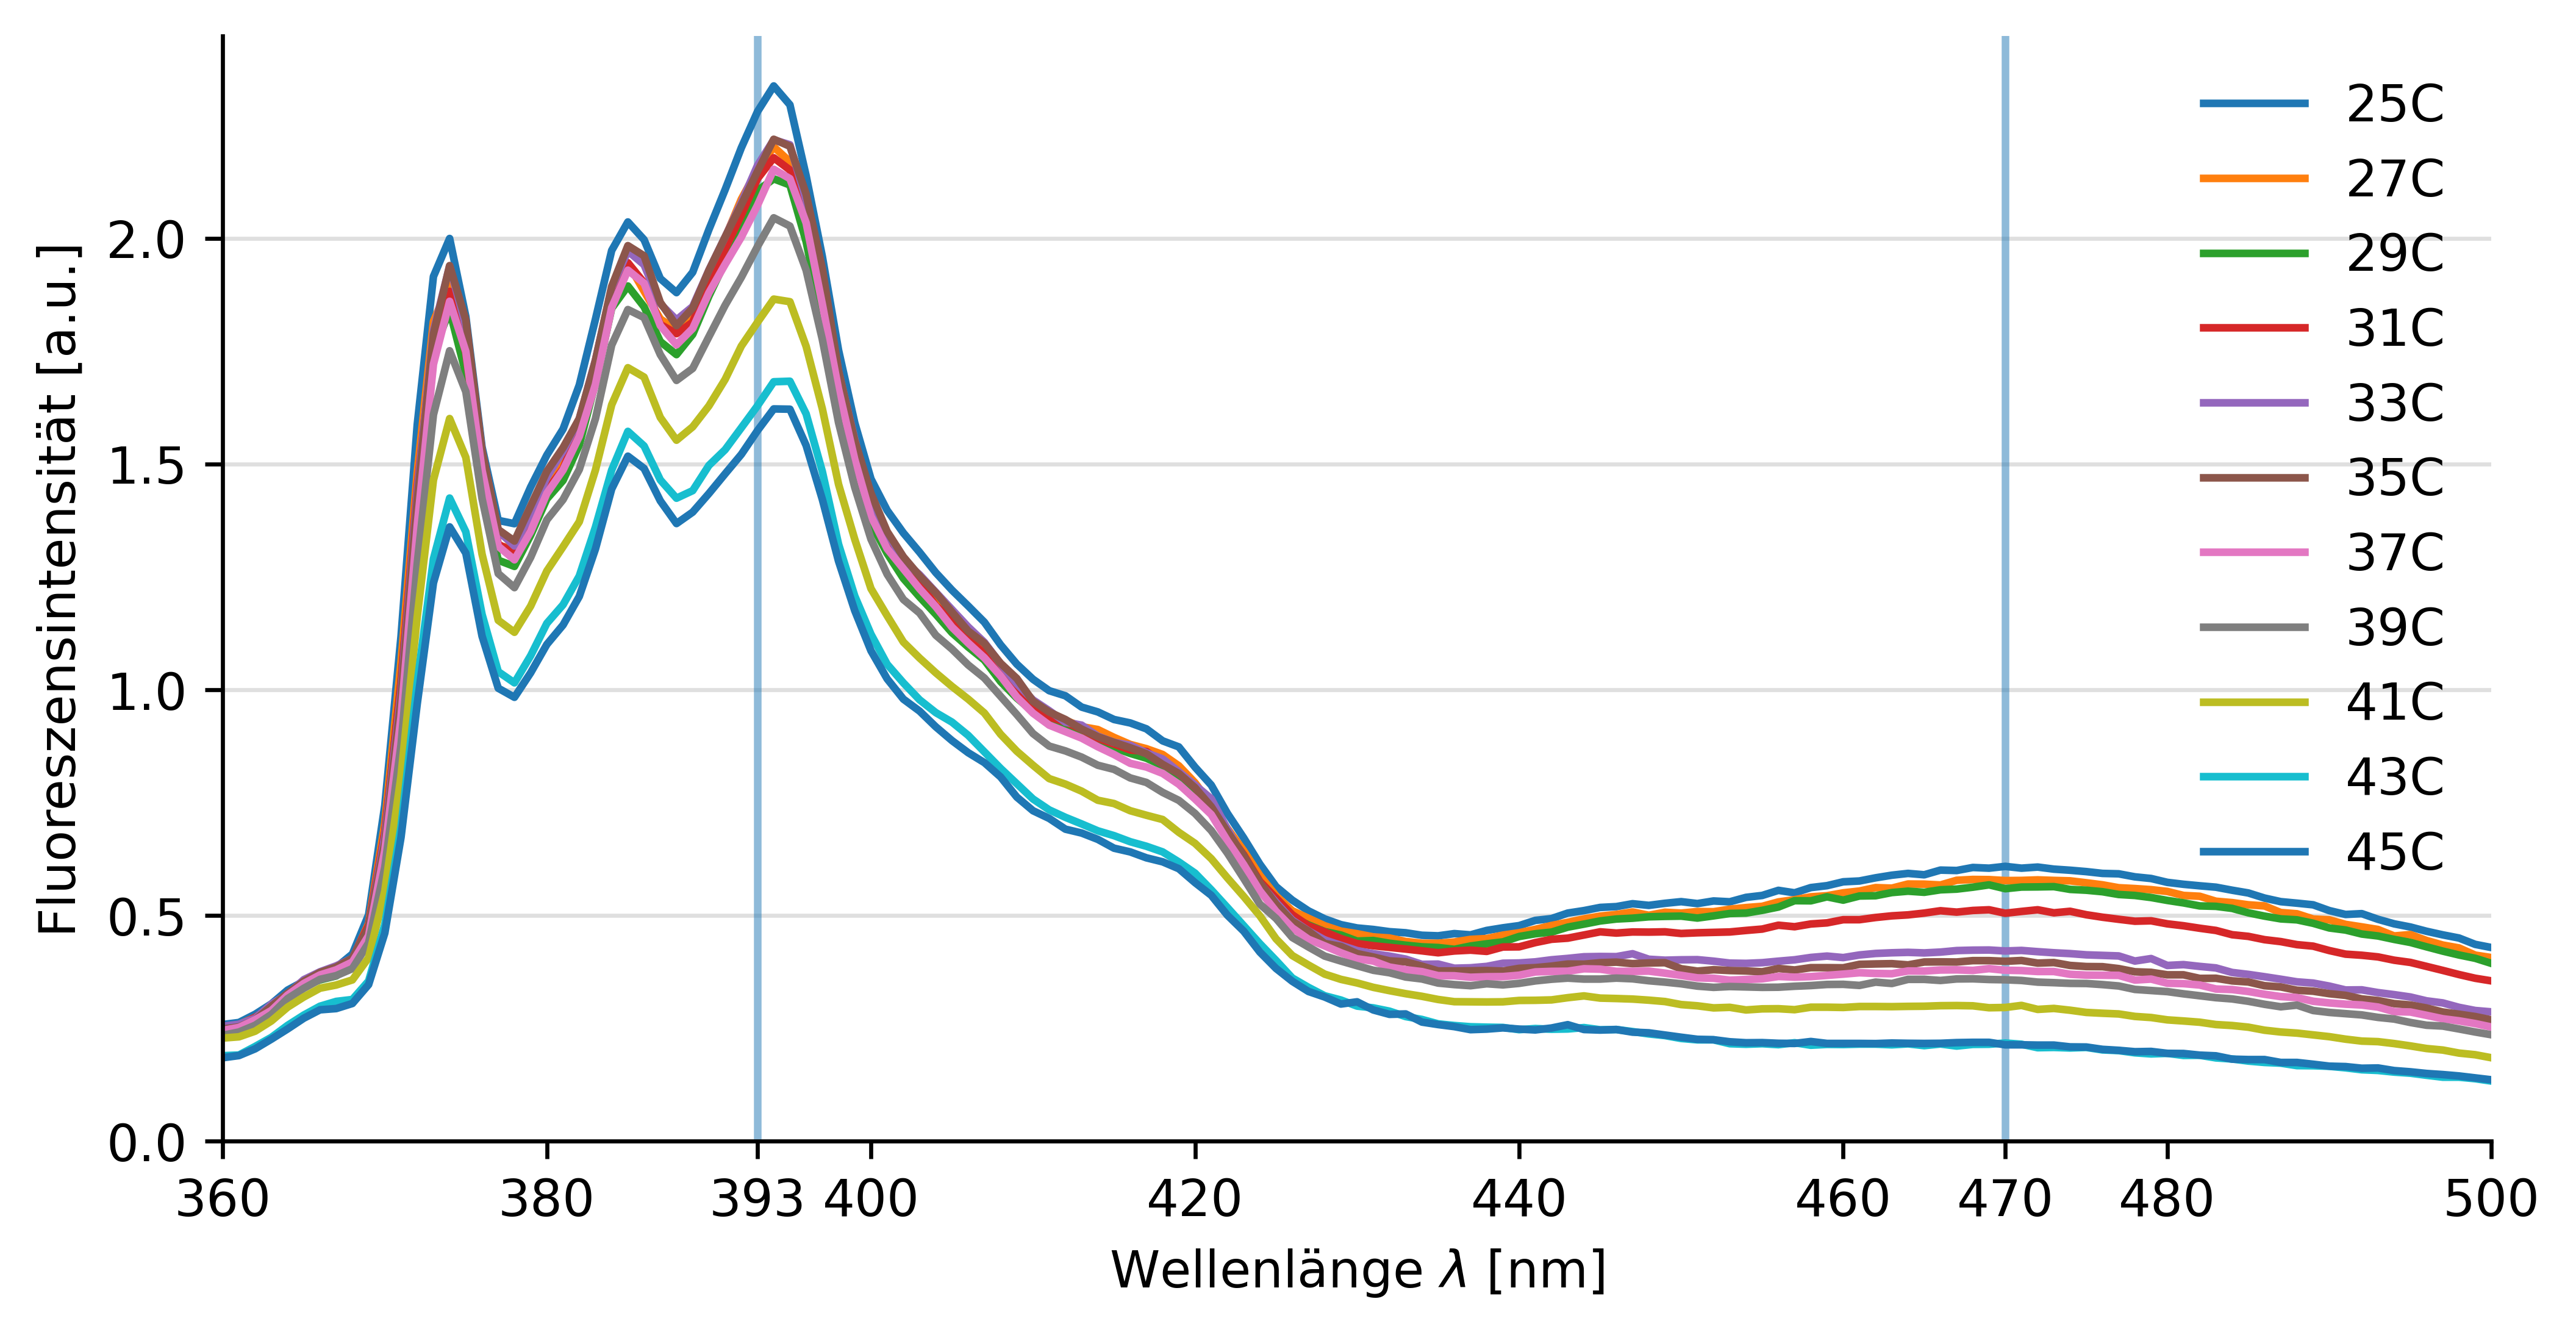
\includegraphics[width=\textwidth]{analysis/reports//Temp_Device4.png}
			\caption{Fluoreszenzintensität Spektrum von Pyren in DPPC; temperaturabhängig} 
			\label{Temp_Geraet4} 
		\end{minipage}
	\end{center}
\end{figure}
\begin{figure}[h!]
	\begin{center}
		\begin{minipage}{0,8\textwidth}
			
			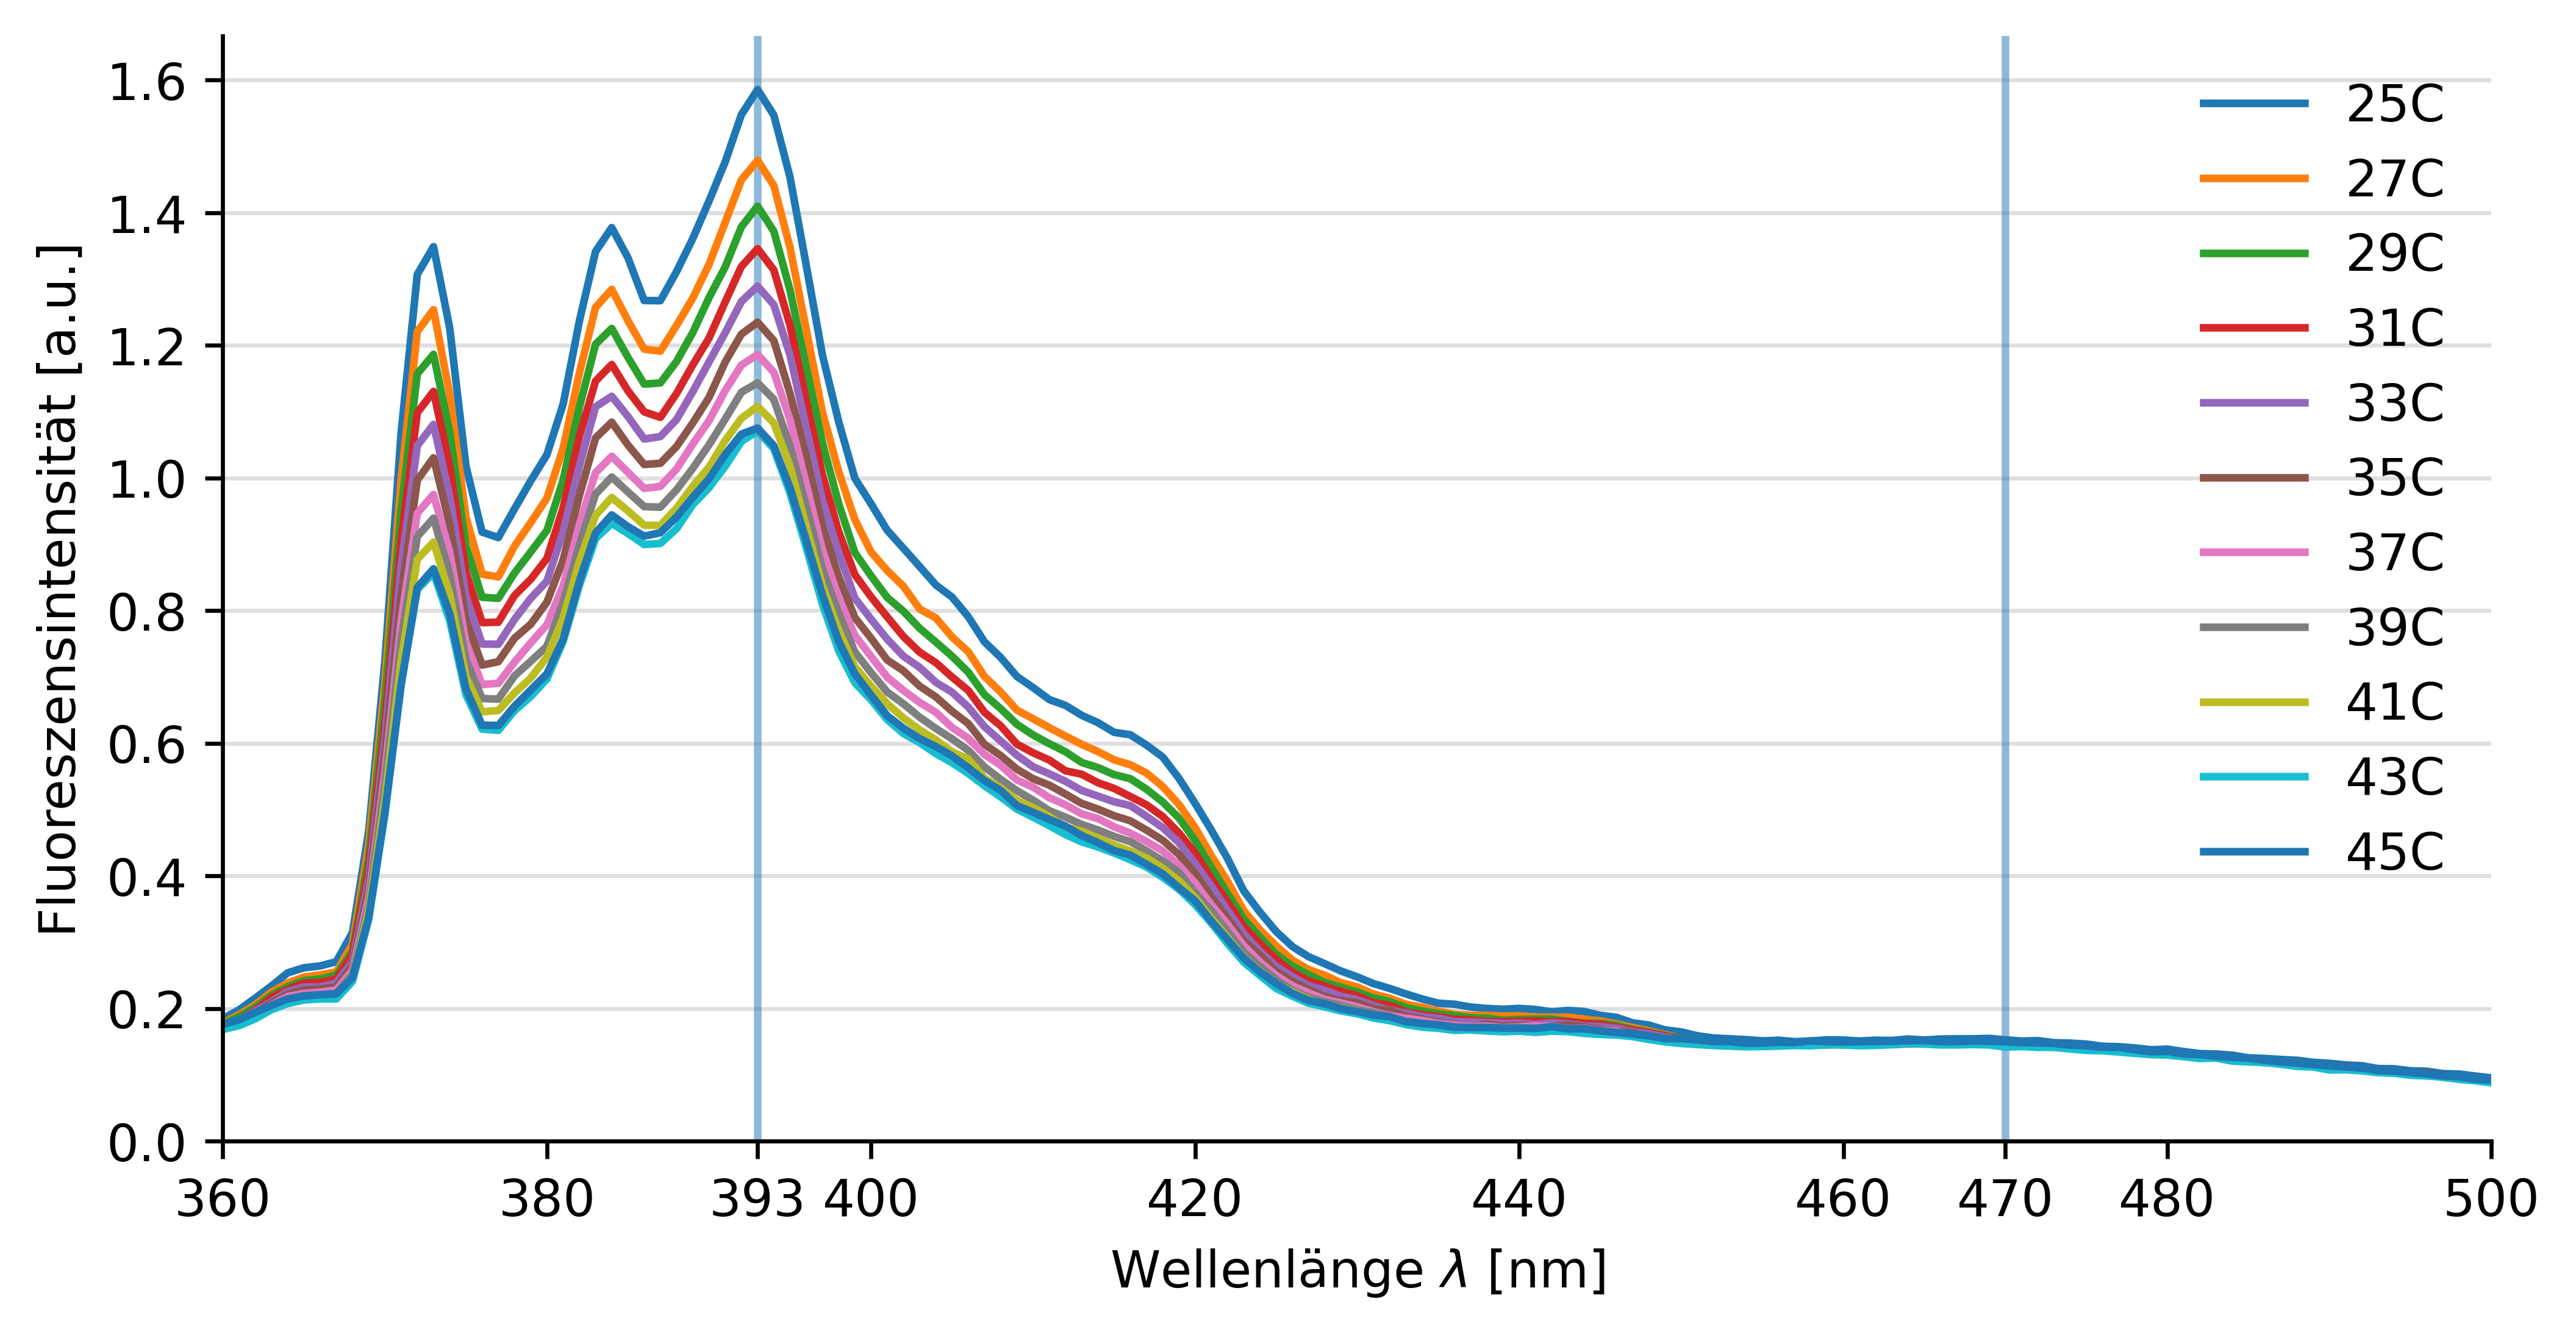
\includegraphics[width=\textwidth]{analysis/reports/Temp_Device3.png}
			\caption{Fluoreszenzintensität Spektrum von Pyren in Ei-PC; temperaturabhängig} 
			\label{Temp} 
		\end{minipage}
	\end{center}
\end{figure}
Eine Einordnung der errechneten $D_{diff}$ von Pyren (Tabelle \ref{tab:meinetabelle}) in die allgemeine Literatur erweißt sich als schwer, da in keinem Buch beziehungsweise Paper entsprechende Versuche mit $D_{diff}$ Daten gefunden wurden. Die Größenordnung von $D_{diff}$ bezüglich Pyren in Ei-PC stimmt aber annäherend mit ähnlichen Versuchen überein. \cite{Wu1977} \\\\
Das Verhältnis Excimer zu Monomer wird durch die Beweglichkeit und  Konzentrationen bestimmt. \cite{Creuwels1996}\\
Die Fluoreszenzlebenszeiten des Excimers $\tau_0$ (Tab. \ref{tab:Lebenszeiten}) nehmen bei steigender Temperatur wohl deshalb ab, da sich die Diffusionsrate durch Zunahme der Membranfluidität erhöht.\\
Die Technik des Versuchs ist nicht für \textit{flip-flop}  Prozesse geeignet, da der empflindliche Frequenzbereich der Fluoreszenzmessung von circa $10^{-10}\text{ bis } 10^{-7}$ s nicht den Frequenzbereich eines Lipid \textit{flip-flop} Prozess von oft mehr als 1min abdecken kann. \\
Zur Berechnung von $D_{diff}$ bedarf  es Fluoreszenzlebenszeiten $\tau_0$, die durch das Skript gestellt wurden. Unter welchen Bedingungen diese gewonnen wurden, wurde nicht erwähnt. Deshalb sind die in der Tabelle \ref{tab:meinetabelle} dargestellten $D_{diff}$ kritisch zu betrachten. Membranproteine, die sich in realen System befinden, können u.a. ein Hindernis für die Lateraldiffusion $D_{diff}$ von Lipiden darstellen und $D_{diff}$ nahe der Proteine beschränken. Außerdem verändern Proteine die Packungsdichte der Lipide, wodurch kleinere Lipiddomaine entstehen. Die im Versuch gemessenen $D_{diff}$ sind somit eher nur quantitativer Natur. \\
%In Abb. \ref{Ex_Mono} bei DPPC sieht man 2 Übergänge. Einen bei $T=35^\circ C$ und einen bei  $T=43^\circ C$. Der Erste kann ein Artefakt sein bzw. vielleicht kann man darin auch die Ripple Phase $P_{\beta '}$ sehen. Eine engmaschigere Messreihe würde für Klarheit sorgen.\\
%Ei-PC  besitzt gegenüber DPPC (16:0) über ungesättigte Fettsäuren mit cis-Bindungen, die eine Störung der Anordnung der Lipide in der Membran darstellen. Ei-PC verbleibt deswegen im flüssig-kristallinen Zustand $L_\alpha$. DPPC wandelt sich von der Gelphase $L_{\beta '}$ ab circa $T=43^\circ C$ in $L_\alpha$ um, was man indirekt aus der Abb. \ref{Ex_Mono} herauslesen kann. Für eine eindeutige Aussage bezüglich der Phasenumwandlung ist die Technik  des vorliegenden Experiment als alleinstehende Methode weniger geeignet. Die möglichen Phasenumwandlungspunkte für DPPC von $L_{\beta '} \rightarrow P_{\beta '}$ und von $P_{\beta '} \rightarrow L_\alpha$ stimmen aber annäherend mit den Literaturwerten von $36^\circ C$ ($L_{\beta '} \rightarrow P_{\beta '}$) und $41.3^\circ C$ ($P_{\beta '} \rightarrow L_\alpha$) überein \cite{Biltonen1993}.\\
Wichtig festzuhalten ist, dass bei den Messungen im Kapitel \ref{sec:FvonT} nicht exakt bei den angeforderten Temperaturmesspunkten gemessen wurde. Dies liegt im Problem der genauen Einstellbarkeit der Temperatur des Messystem, da die eingestellte Temperatur seltens wirklich erreicht wurde. Deshalb wurde so verfahren, dass, wenn keine Temperaturveränderung nach 2min mehr gemessen wurde, die jeweilige Messung erfollgte, auch wenn bis dahin nicht die eingestelle neue Temperatur erreicht wurde. Dadurch entstand auch ein Fehler, dass nunmehr die Daten nicht zu den angegebenen $\tau_0$ Messwerten aus der Tabelle \ref{tab:Lebenszeiten} passen, wodurch sich die Berechnung von  $D_{diff}$ weiter verfälscht.

%\newpage